
\documentclass{article}
\usepackage[utf8]{inputenc}
\usepackage{graphicx}
\usepackage{listings}
\usepackage{xcolor}
\usepackage{float}  % Add float package to control figure placement
\usepackage{amsmath}

\title{09b Keypad-Piezo Buzzer Alarm Introduction}
\author{Nicholas Bruzzese}
\date{\today}

\definecolor{dkgreen}{rgb}{0,0.6,0}
\definecolor{gray}{rgb}{0.5,0.5,0.5}
\definecolor{mauve}{rgb}{0.58,0,0.82}

\lstset{frame=tb,
	language=Python,
	aboveskip=3mm,
	belowskip=3mm,
	showstringspaces=false,
	columns=flexible,
	basicstyle={\small\ttfamily},
	numbers=none,
	numberstyle=\tiny\color{gray},
	keywordstyle=\color{blue},
	commentstyle=\color{dkgreen},
	stringstyle=\color{mauve},
	breaklines=true,
	breakatwhitespace=true,
	tabsize=3
}

\begin{document}
	
	\maketitle
	
	\section*{Introduction}
	This project teaches you how to create an alarm system with a buzzer and a 4x4 keypad connected to a Raspberry Pi. The system activates the buzzer after a random delay, and it can only be deactivated by entering the correct PIN code on the keypad.
	
	\section*{Objectives}
	By the end of this lesson, you will:
	\begin{enumerate}
		\item Understand how to interface a buzzer and keypad with a Raspberry Pi.
		\item Learn to use GPIO pins for input (keypad) and output (buzzer).
		\item Build a Python program to control the alarm system.
	\end{enumerate}
	
	\section*{Hardware Setup}
	\subsection*{Components}
	\begin{itemize}
		\item Raspberry Pi (any model with GPIO pins).
		\item 4x4 keypad.
		\item Piezo buzzer.
		\item Jumper wires.
	\end{itemize}
	
	\section*{Wiring Diagram}
	\begin{figure}[H]
		\centering
		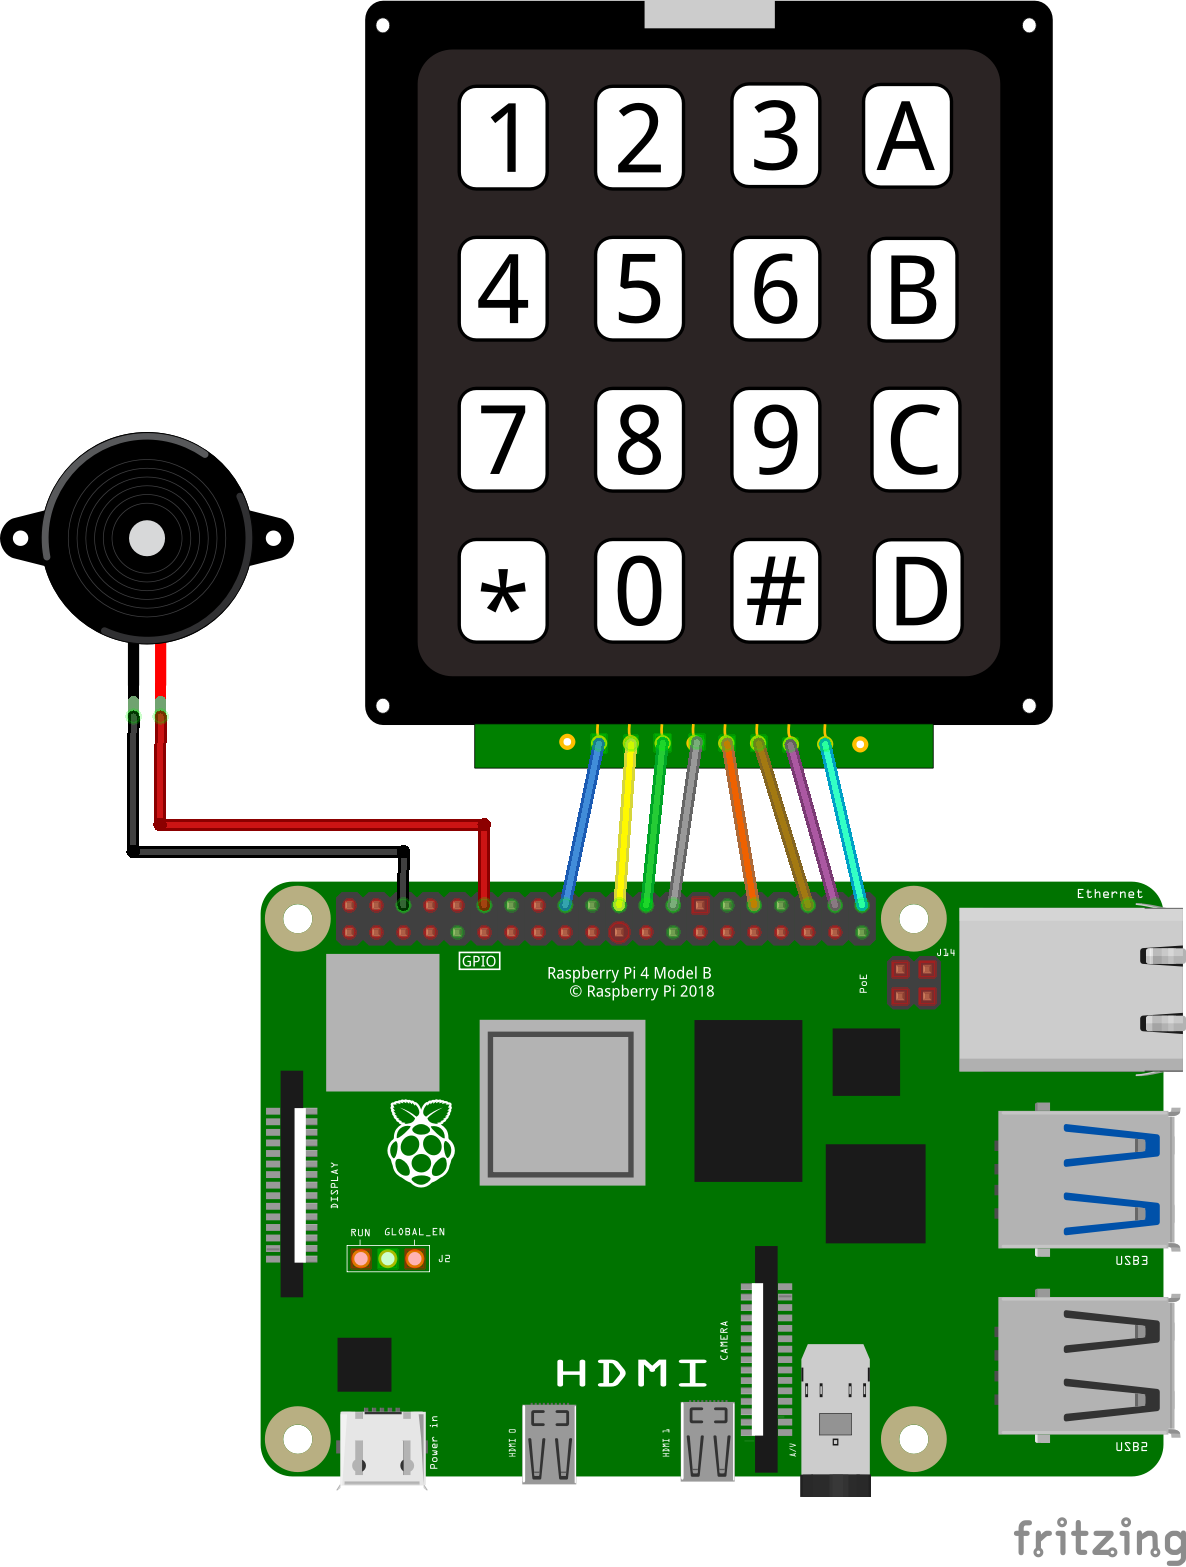
\includegraphics[width=0.8\textwidth]{09b-keypad-piezo.png} % Adjust width to 80% of text width
		\caption{Wiring Diagram}
	\end{figure}
	
	\newpage
	\subsection*{Connections}
	\textbf{Keypad}: Connect the rows (R1–R4) and columns (C1–C4) of the keypad to the GPIO pins as follows:
	
	\begin{center}
		\begin{tabular}{|l|l|}
			\hline
			\textbf{Keypad Pin} & \textbf{GPIO Pin} \\
			\hline
			R1 & GPIO 24 \\
			R2 & GPIO 25 \\
			R3 & GPIO 8  \\
			R4 & GPIO 7  \\
			C1 & GPIO 12 \\
			C2 & GPIO 16 \\
			C3 & GPIO 20 \\
			C4 & GPIO 21 \\
			\hline
		\end{tabular}
	\end{center}
	
	\textbf{Buzzer}: Connect the positive terminal to GPIO 18 and the negative terminal to GND.
	
	
	\section*{Code Explanation}
	Below is the Python code, along with explanations for each section:
	
	\subsection*{1. GPIO Initialization}
	This section sets up the GPIO pins for the keypad and buzzer:
	\begin{itemize}
		\item Rows (R1–R4) are configured as output.
		\item Columns (C1–C4) are configured as input with pull-down resistors to detect button presses.
		\item The buzzer pin is configured as output.
	\end{itemize}
	
	\begin{lstlisting}
		# GPIO pin definitions for keypad
		L1 = 24
		L2 = 25
		L3 = 8
		L4 = 7
		C1 = 12
		C2 = 16
		C3 = 20
		C4 = 21
		
		# GPIO pin for the buzzer
		BUZZER = 18
		
		# Initialize GPIO
		GPIO.setwarnings(False)
		GPIO.setmode(GPIO.BCM)
		
		# Setup keypad GPIO pins
		GPIO.setup([L1, L2, L3, L4], GPIO.OUT)
		GPIO.setup([C1, C2, C3, C4], GPIO.IN, pull_up_down=GPIO.PUD_DOWN)
		
		# Setup buzzer GPIO pin
		GPIO.setup(BUZZER, GPIO.OUT)
	\end{lstlisting}
	
	\subsection*{2. Buzzer Control}
	The \texttt{buzz} function turns the buzzer ON or OFF by setting the output state of the buzzer GPIO pin.
	
	\begin{lstlisting}
		def buzz(state):
		"""Turn the buzzer on or off."""
		GPIO.output(BUZZER, state)
	\end{lstlisting}
	
	\subsection*{3. Keypad Scanning}
	The \texttt{read\_line} function scans a single row of the keypad by activating the row and checking the state of each column. If a column input is HIGH, it means the corresponding key is pressed.
	
	\begin{lstlisting}
		def read_line(line, characters):
		"""Read input from the keypad."""
		GPIO.output(line, GPIO.HIGH)
		if GPIO.input(C1) == 1:
		process_key(characters[0])
		if GPIO.input(C2) == 1:
		process_key(characters[1])
		if GPIO.input(C3) == 1:
		process_key(characters[2])
		if GPIO.input(C4) == 1:
		process_key(characters[3])
		GPIO.output(line, GPIO.LOW)
	\end{lstlisting}
	
	\subsection*{4. Processing Key Presses}
	The \texttt{process\_key} function handles key presses. If the alarm is active:
	\begin{itemize}
		\item It appends the key to the \texttt{input\_code}.
		\item Checks if the entered code matches the preset \texttt{PIN\_CODE}.
		\item If correct, it turns off the buzzer and deactivates the alarm. If incorrect, it resets the code and prompts the user to try again.
	\end{itemize}
	
	\begin{lstlisting}
		def process_key(key):
		"""Handle key press events."""
		global input_code, alarm_active
		
		if alarm_active:  # Only process keys if the alarm is active
		print(f"Key pressed: {key}")
		input_code += key
		
		if len(input_code) >= len(PIN_CODE):  # Check PIN code
		if input_code == PIN_CODE:
		print("Correct PIN entered. Alarm deactivated.")
		buzz(False)  # Turn off the buzzer
		alarm_active = False
		else:
		print("Incorrect PIN. Try again.")
		input_code = ""  # Reset the entered PIN
	\end{lstlisting}
	
	\subsection*{5. Main Program}
	The program starts by initializing the alarm system and waits for a random delay before activating the buzzer. The main loop continuously checks the keypad for key presses.
	
	\begin{lstlisting}
		try:
		# Main program loop
		print("System initialized. Waiting for alarm...")
		time.sleep(random.randint(5, 15))  # Random delay before alarm activates
		print("ALARM TRIGGERED!")
		buzz(True)  # Activate the buzzer
		alarm_active = True
		
		while True:
		# Continuously check the keypad
		read_line(L1, ["1", "2", "3", "A"])
		read_line(L2, ["4", "5", "6", "B"])
		read_line(L3, ["7", "8", "9", "C"])
		read_line(L4, ["*", "0", "#", "D"])
		time.sleep(0.1)
		
		except KeyboardInterrupt:
		print("\nApplication stopped!")
		
		finally:
		GPIO.cleanup()
	\end{lstlisting}
	
	\section*{How It Works}
	\begin{enumerate}
		\item The program initializes and waits for a random delay (5–15 seconds).
		\item The buzzer activates, simulating an alarm.
		\item The user must input the correct PIN code on the keypad to deactivate the alarm.
		\item If the correct code is entered, the buzzer stops, and the system resets.
	\end{enumerate}
	
	\section*{Exercises}
	\begin{itemize}
		\item \textbf{Change the PIN Code}: Modify the \texttt{PIN\_CODE} variable to set a new PIN.
		\item \textbf{Add More Features}: Display instructions on an LCD or add an LED indicator for alarm status.
		\item \textbf{Custom Sounds}: Use a passive buzzer to play custom alarm tones.
	\end{itemize}
	
	This project is a great introduction to using GPIO pins for both input and output on a Raspberry Pi. Experiment with additional features to enhance the system! Let me know if you need help expanding this project.
	
\end{document}
